\documentclass[a4paper,10pt, sans]{article}
\usepackage[utf8x]{inputenc}
\usepackage[spanish]{babel}
\usepackage{hyperref}
\usepackage{verbatim}
\usepackage{graphicx}
\usepackage{float}
\usepackage{wrapfig}
\usepackage{ltxtable}
%\usepackage{amsmath,amssymb,amsfonts,latexsym,cancel}
\usepackage{multicol}      %para usar varias columnas
  %uso:
  %\begin{multicols}{2}
    %texto
  %\end{multicols}
\usepackage{marvosym}

\setlength{\columnsep}{4mm}    %separación de columnas
%\usepackage{pslatex}
%\hoffset -0.75in        %cambio el margen horizontal izquierdo
%\voffset -0.9in          %cambio el margen vertical superior
\textwidth 17cm        %ancho de texto. defaut: 14cm
\textheight 25cm        %alto de texto. default: 19cm
\topmargin -1cm        %agranda el margen superior. default: 3cm
\oddsidemargin -1cm        %agranda el margen izquierdo. default: 2.5cm (4.5 si no aparece esta instrucción)
\pagestyle{empty} %{myheadins}  %numeración de pág: sin / arriba
\parskip 2mm          %X mm entre párrafos
%\parindent 0mm          %elimina sangría

\begin{document}
  

  \begin{wrapfigure}{r}{4cm}
    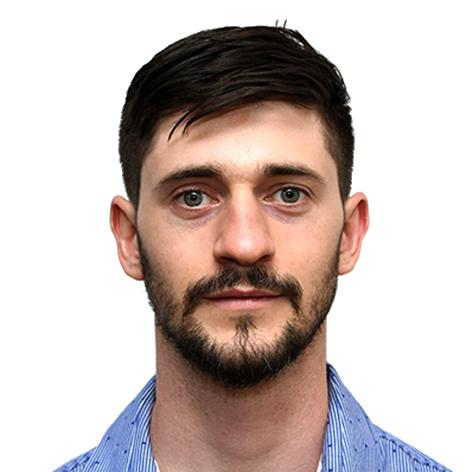
\includegraphics[height=4cm]{seba_4x4.jpg}
  \end{wrapfigure}

  \sffamily
  
  \begin{Huge}
    Sebastián Rossi
  \end{Huge}
  \\ \\
  \hspace*{0.5cm} \textit{CURRICULUM VITAE} \\
  \hspace*{0.5cm} {\textit{Actualizado: 25/04/2025}}
  
  \begin{tabular}{rl}
    \vspace{0.5cm} \\
    \large\Mobilefone & \textbf{+549 3402 507471} \\
    \large\Letter & \textbf{srossi@inti.gob.ar} \\
    {} & \textbf{sbstnrossi@outlook.com}
  \end{tabular}

  \vspace{0.5cm}
  \large
  \begin{table}[h!]
  \begin{tabularx}{\textwidth}{r X}
    %%%%%%%%%%%%%%%%%%%%%%%%%%%%%%%%%%%%%%%%%%%%%%%%%%%%%%%%%%%%%%%%%%%%%%%%%%%%
    \textbf{Datos} & {}  \\ [1ex]
      \textbf{Personales} & Fecha de Nacimiento: 15-11-1988 \\ [1ex]
      {} & Nacionalidad: Argentino - Italiano \\ [1ex]
      {} & Domicilio: Maipú 782, (2107) Álvarez, Santa Fe, Argentina \\ \\ \hline \\

    %%%%%%%%%%%%%%%%%%%%%%%%%%%%%%%%%%%%%%%%%%%%%%%%%%%%%%%%%%%%%%%%%%%%%%%%%%%%
    
    \textbf{Educación} & {} \\ [1ex]
       (2020 - ) & \textbf{Doctorado en Ingeniería}, FCEIA, Universidad Nacional de Rosario. Tesis: Sensado y control de sistemas de siembra neumáticos. Directores: Ignacio Rubio Scola, Gastón Bourges.\\ [1ex]
       (2008 - 2014) & \textbf{Ingeniero Electrónico}. FCEIA, Universidad Nacional de Rosario.\\ \\ \hline \\
    %%%%%%%%%%%%%%%%%%%%%%%%%%%%%%%%%%%%%%%%%%%%%%%%%%%%%%%%%%%%%%%%%%%%%%%%%%%%
    \textbf{Antecedentes} & \textbf{Laborales} \\ [1ex]
      (2013 - ) & Instituto Nacional de Tecnología Industrial. Departamento de Ingeniería de Productos Industriales - Rosario.\\ \\
            
        {} & \hspace{2cm} \textit{Desarrollo de nuevas capacidades.} \\ [1ex]
        
        (2013) & Medición de distribución de temperatura y tiempos de estabilización térmica en laboratorio de calibración de bloques patrón. \\ [1ex]
        (2013 - 2014) & Desarrollo de software para la adquisición de datos por puerto serie de comparadora de bloques patrón. \\ [1ex]
        (2014 - 2015) & Desarrollo e implementación de sistema de grabación multicanal comandado por wi-fi con placas Raspberry-Pi. Aplicación: detección de impacto de semillas. \\ [1ex]
        (2015) & Desarrollo de scripts en Scilab para determinar el tiempo de impacto de diferentes tipos de semillas a partir de señales de sensores piezoeléctricos y evaluación de sistemas de siembra según norma ISO 7256. \\ [1ex]
        (2016) & Desarrollo de plataforma basada en Cortex M4 para múltiples canales sincronizados de sensado para detección de impacto de semillas. \\ [1ex]
        (2016 - 2017) & Redacción de documentación para integrar el servicio de medición de deformaciones con galgas extensiométricas al sistema de gestión de calidad. \\ [1ex]
        (2017 - 2019) & Experimentación en banco de pruebas air-drill con diferentes niveles de caudal de aire, flujo de semillas, configuración de cabezal distribuidor y longitudes de mangueras de salida con semillas de soja. \\ [1ex]
        (2018) & Desarrollo de plataforma modular basada en Cortex M0 con comunicación inalámbrica para adquisición de datos multicanal para sensores piezoeléctricos y transmisores de presión. \\ [1ex]
        (2019 - 2020) & Desarrollo de software de procesamiento de imágenes en python usando la biblioteca OpenCV para detección de trayectorias de semillas en videos de alta velocidad para evaluacion de dosificadores de siembra de precisión y tubos de descarga de semillas en banco de pruebas sobre mesa vibradora. Scripts R para el análisis de los resultados. \\ [1ex]
        (2020 - 2023) & Experimentos en banco de pruebas estático y análisis de los datos para evaluación de incertidumbre en sistemas de detección de semillas y trayectorias mediante placa de impacto, sensores infrarrojos y procesamiento de imágenes.
       
  \end{tabularx}
  \end{table}
  
  \begin{table}[H]
  \centering
  \begin{tabularx}{\textwidth}{r X}
        (2023) & Capacitación dictada a 2 becarios en pegado y conexionado de galgas extensiométricas. \\ [1ex]
        (2023 - ) & Arreglo de sensores ópticos en 2 ejes para detección de paso de semillas. Método de detección implementado en placa de desarrollo con ESP32. \\ [1ex]
        (2024) & Programación de microcontrolador ESP32 para control de banco de ensayos de
dosificadores de siembra y adquisición de datos del sistema. \\ [1ex]
        (2024) & Programación de PLC para bancos de ensayos de evaluación de protecciones en barras cardánicas.\\ [1ex]
        (2025) & Experimentos en banco de pruebas estático y análisis de los datos para evaluación de incertidumbre en sistemas de detección de semillas con arreglo de sensores ópticos en 2 ejes.\\ \\
        
        
        
        
        {} & \hspace{2cm} \textit{Trabajos realizados para usuarios.} \\ [1ex]
        (2015 - 2016) & Evaluación de una sembradora a chorrillo usando detección de semillas con sensores piezoeléctricos tanto en banco de pruebas como sembrando en campo, basado en ISO 7256 Parte 2. Empresa: Indecar. \\  [1ex]

        (2015 - ) & Evaluación de dosificadores de siembra de precisión y tubos de descarga de semillas con procesamiento de imágenes y sensor piezoeléctrico basado en ISO 7256 Parte 1, en banco de ensayos estático y dinámico. Empresas: Siembra Neumática, Pla, Agrometal. \\ [1ex]
        (2016 - ) & Pegado de galgas extensiométricas y medición de deformaciones en estructuras de acero. Empresas: Acerías 4C, Agrometal, Crucianelli, Ejército Argentino, Hermann, Juri, Ombú, Palfinger, Pla, Randon, Sola y Brusa, Superwalter, Tandanor. \\ [1ex]
        (2023 - ) & Transferencia tecnológica de sistema de detección de paso de semilla para banco de ensayos estático de dosificador de presición en fábrica. Empresa: Siembra Neumática. \\ [1ex]
        (2024)&  Filmación de alta velocidad para medición de velocidad de caida en máquina de ensayos de punteras de calzado de seguridad y estimación de incertidumbres para la empresa Maincal. \\ [1ex]
        (2024 - 2025) & Medición de torque en eje de dosificadores de siembra de precisión para la empresa
Abelardo Cuffia. \\ \\ \hline \\

    \textbf{Publicaciones } & {} \\ [1ex]
    {Revistas} & {Rossi, S., Rubio Scola, I., Bourges, G., Sarauskis, E., Karayel, D. (2023) \textit{Improving the seed detection accuracy of piezoelectric impact sensors for precision seeders. Part I: A comparative study of signal processing algorithms}. Computers and Electronics in Agriculture. Vol 215. 108449.} \\ [1ex]
      {} & {Rossi, S., Rubio Scola, I., Bourges, G., Sarauskis, E., Karayel, D. (2023) \textit{Improving the seed detection accuracy of piezoelectric impact sensors for precision seeders. Part II: Evaluation of different plate materials}. Computers and Electronics in Agriculture. Vol 215. 108448.} \\ [1ex]
    {Capítulo de libro} & Rubio Scola, I., Rossi, S., Bourges, G. \textit{Air drill Seeder Distributor Head Evaluation: A Comparison between Laboratory Tests and Computational Fluid Dynamics Simulations.} Capítulo de libro: Information and Communication Technologies for Agriculture — Theme II: Data. \\ [1ex]
    Congresos & Bourges, G., Rossi, S., Eliach, J., Medina, M. \textit{Evaluación experimental de un dosificador de semillas de precisión.} V CAIM 2016. Santiago del Estero, Argentina. UNSE- FCEyT- ISBN: 978-987-1676-63-7. pp: 881-891. \\  [1ex]
      {} & Rossi, S., Rubio Scola, I., Eliach, J., Bourges, G. \textit{Evaluación de desempeño de dosificador monograno mediante filmación y procesamiento de imágenes.} VII CAIM 2020. San Nicolás, Argentina. \\  [1ex]
      {} & Bourges, G., Rossi, S., Rubio Scola, I., Karayel, D. \textit{Evaluación de la incidencia de diferentes factores en la distribución de semillas de soja en sistema de transporte por aire.} VII CAIM 2020. San Nicolás, Argentina. \\  [1ex]
      {} & Rossi, S., Rubio Scola, I., Bourges, G., Eliach, J., Šarauskis, E., Karayel, D. \textit{Improving seed detection accuracy with infrared sensors array in precision seeders}. VIII CAIM 2023. Santa Fe, Argentina. \\  [1ex]
     
  \end{tabularx}
  \end{table}



  
  \begin{table}[H]
  \centering
  \begin{tabularx}{\textwidth}{r X}  
     
      {} & Davut Karayel, Eglė Jotautienė, Egidijus Šarauskis, Sebastián Rossi, Ignacio Rubio Scola, Gastón Bourges. \textit{EVALUATION OF MONITORING SYSTEMS FOR SEEDER SEED SPACING UNIFORMITY}. Journal of International Scientific Publications: Agriculture \& Food 12, 105-116 (2024). https://doi.org/10.62991/AF1996556881  \\  [1ex]
      {} & Sebastián Rossi, Ignacio Rubio Scola, Gastón Bourges, Jorge Eliach, Egle Jotautiene,
Egidijus Šarauskis, Davut Karayel. \textit{Piezoelectric impact sensor and infrared array sensor:
comparative study for precision seeders}. Ibersensor 2024. \\ \\ \hline \\
    

\textbf{Cursos} & {}\\ [1ex]
    
      {} & Evaluación de incertidumbre de medición. 16 h. INTI Rosario. \\ 
      {} & Solidworks. 24 h. Disegno Soft SRL. \\
      {} & Análisis de vibraciones, categoría II, ISO 18436-2. 38 h. Semapi Argentina S.A.\\
      {} & Programación de microcontroladores PIC en lenguaje C. 30 h. Escuela de posgrado de la FCEIA, UNR. \\
      {} & Síntesis de sistemas digitales en FPGA. 30 h. Escuela de posgrado de la FCEIA, UNR. \\
      {} & RTOS sobre microcontroladores de 32 bits. 30 h. Escuela de posgrado de la FCEIA, UNR. \\
      {} & Diseño de experimentos. 30 h. Escuela de posgrado de la FCAGR, UNR. \\
      {} & Análisis multivariado. 50 h. Escuela de posgrado de la FCAGR, UNR. \\
      {} & Introducción al diseño y análisis de experimentos industriales. 38 h. Escuela de graduados y extensión universitaria de la FCECON, UNR. \\
      {} & Procesamiento digital de imágenes. 70 h. Escuela de posgrado de la FCEIA, UNR. \\
      {} & Modelado y simulación de sistemas dinámicos. 70 h. Escuela de posgrado de la FCEIA, UNR. \\ \\ \hline \\
    
\textbf{Idiomas} & {} \\ [1ex]
    {} & Español, lengua madre. \\ [1ex]
    {} & Inglés, Nivel intermedio. \\ \\ \hline \\
      
    \textbf{Licencia de} & {} \\ [1ex]
    \textbf{conducir} & Clases A3 y B2.\\
    
\vspace{5cm}
    
    
    
    
        
  \end{tabularx}
  \end{table}
  
\end{document}
